%!TEX root = GRoutes.tex
%%%%%%%%%%%%%%%%%%%%%%%%%%%%%%%%%%%%%%%%%%%%%%%%%%%%%%%%%%%%%%%%%%%%%%%
\chapter{GRoutes - alkalmazás bemutatása}\label{ch:ALAP}
%%%%%%%%%%%%%%%%%%%%%%%%%%%%%%%%%%%%%%%%%%%%%%%%%%%%%%%%%%%%%%%%%%%%%%%

\begin{osszefoglal}
	Ebben a fejezetben a GRoutes android applikációt fogom bemutatni úgy technikai, mint funkcionális szempontból.
	
\end{osszefoglal}

%%%%%%%%%%%%%%%%%%%%%%%%%%%%%%%%%%%%%%%%%%%%%%%%%%%%%%%%%%%%%%%%%%%%%%%
\section{Funkcionalitások}\label{sec:ALAP:adatelem}

\subsection{Bejelentkezés}

\begin{wrapfigure}{l}{0.4\linewidth}
	\centering
	\setlength{\abovecaptionskip}{0pt}
	\setlength{\belowcaptionskip}{0pt}
	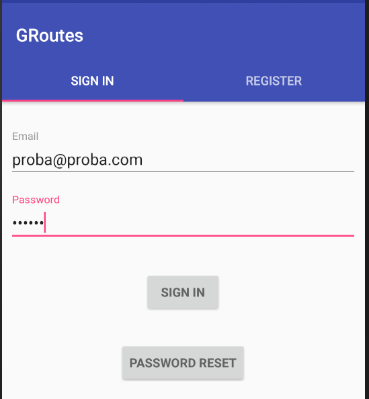
\includegraphics[width=0.4\textwidth]{images/login}
	\caption{Bejelentkezési felület\label{fig:ALAP:sm2}}
\end{wrapfigure}

Az alkalmazás elindítása után egy bejelentkezési felület fogadja a felhasználót. Itt kell megadni az e-mail címet, valamint a jelszót amivel a felhasználó regisztrált. Amennyiben elfelejtette a jelszavát, az "elfelejtett jelszó" gomb megnyomásával lehetőség van egy jelszó-visszaállító e-mail kiküldésére. 



Ha egy új felhasználó szeretné igénybe venni az applikáció szolgáltatásait, akkor regisztrálnia kell. Ezt megteheti a regisztráció lapra való navigálás után, melyet a cím megérintésével, vagy a képernyőn az ujjának balra történő húzásával érheti el. Az e-mail cím és az új jelszó megadása után, a felhasználó egyből a főmenübe érkezik, mindeközben azonban egy aktivációs e-mailt is kap arra a címére, amivel regisztrált. A későbbiekben csak akkor fog tudni bejelentkezni, ha a kapott emailben az URL%
\footnote{ %
	Uniform Resource Locator, más néven webcím
}  %
-re klikkelve aktiválja a felhasználóját.

\subsection{Főmenü}

A fomenubol negy kulonbozo oldalra navigalhatunk tovabb: a keresesi felulet, a regebbi keresesek megtekintese, a kedvencek menedzselese valamint a beallitasok.
Az otodik (csoportok) oldal egy jovobeli funkcionalitas kifejlesztesere van fenntartva.

\subsection{Keresési felület}
A keresesi felulet

\subsection{Térkép felület}

Terkep felulet
Ez a felulet akkor jelenik meg, amikor megerintjuk a terkep gombot egy helyszin vagy egy elmentett utvonal mellett, valamint a keresesi felulet eredmenye is itt jelenik meg.
Amennyiben egy helyintol erkezunk, megjelenik egy jelzo (marker) az adott koordinatan.
A csillag gomb segitsegevel hozzaadhatunk egy utvonalat a kedvencek koze, ahol kesobb modosithatjuk a nevet.

\subsection{Múltbeli keresések}
A multbeli keresesek felulete

A keresesi felulet eredmenyeul kapott utvonalak megjelennek a multbeli keresesek menupont alatt.
Alapertelmezetten a bejegyzesek neve a keresesi datum es idopont lesy. 
Az X gombot megerintve torolhetunk egy bejegyzest, ezaltal az adatbazisbol is torlodni fog.
A terkep gomb megjeleniti a terkep feluletet, ahol kirajzolodik az utvonal. Ez a felulet a fentebb emlitett funkcionalitasokkal rendelkezik.


\subsection{Kedvencek}
A kedvencek felulet

Itt harom muveletet hajthatunk vegre, mindegyiknek megfelel egy gomb.

\subsection{Beállítások}
Beallitasok

Itt ki tudjuk valasztani a limitet, hogy mennyi csomopont eseten melyik algoritmust hasynalja az alkalmazas.
A megadott szamnal kisebb vagy egyenlo szamu csomopontok eseten a Concorde-nevu egzakt megoldasokat nyujto algoritmus fogja kicsamolni az idealis utvonalat.
Ez az algoritmus a legpontosabb megoldasokat nyujtja, azonban az utazo ugynok problemajanak komplexitasa miatt, a csomopontok novekedesevel, a vegrehajtasi ido exponentialisan novekszik.
Amennyiben a felhasznalo nagyon sok csomoponttal szeretne dolgozni es fontosabb neki az hogy belathato idon belul egy elfogadhato megoldast kapjon, de nem problema ha nem a leghatekonyabb utvonal rajzolodik ki,
akkor a megadott szam feletti mennyisegu csomopontok eseten ay applikacio egy ugynevezett greedy algoritmust fog hasznalni, amely polinomialis komplexitassal rendelkezik, ez nagysagrendekkel gyorsabb az exponencialioshoz viszonyitva.

Ugyanitt megadhatjuk az alapertelmezett utazasi modot, ami lehet gyaloglas, valamint vezetes.

Bar az egyszeruseg kedveert igyekeztem sok iras helyett szimbolumokat tenni a gombokra, de az applikacioban talalhato keves szovegnek a nyelvet szinten itt lehet beallitani.

%%%%%%%%%%%%%%%%%%%%%%%%%%%%%%%%%%%%%%%%%%%%%%%%%%%%%%%%%%%%%%%%%%%%%%%
\section{Adatbázis}\label{sec:ALAP:adatelem}

%%%%%%%%%%%%%%%%%%%%%%%%%%%%%%%%%%%%%%%%%%%%%%%%%%%%%%%%%%%%%%%%%%%%%%%
\section{Osztályok}\label{sec:ALAP:adatelem}

%%%%%%%%%%%%%%%%%%%%%%%%%%%%%%%%%%%%%%%%%%%%%%%%%%%%%%%%%%%%%%%%%%%%%%%
\section{Felmerülő problémák}\label{sec:ALAP:adatelem}

